\chapter{Results and interpretation\label{sec:results}}

This chapter presents the final results of the search after the signal region is unblinded, followed by the interpretation of these results in terms of a model-independent limit on the branching ratio Br($H\rightarrow$$aa$$\rightarrow4\tau$).

\section{Observed and expected results\label{sec:results-obsexp}}

Table~\ref{tab:results} shows the expected numbers of signal events from each generated pseudoscalar mass point in each of the $M_{\text{T}}$ bins, followed by the background prediction (obtained from Region B data) and the actual number of events observed in Region A data for $m_{\mu+\text{had}}$ $>$ 4 GeV.

\begin{table*}[htbh]
\begin{center}
\caption{Observed data, estimated background, and expected signal from each generated pseudoscalar mass point in each of the $M_{\text{T}}$ bins assuming SM cross sections and 100\% Br($H\rightarrow$$aa$$\rightarrow4\tau$)  Only statistical error is shown for the signal, while the full error is shown for the background.\label{tab:results}}
\singlespacing
\begin{tabular}{|c|c|c|c|}
\hline
\multicolumn{2}{|c|}{} & $M_{\text{T}} \le$ 50 GeV & $M_{\text{T}} >$ 50 GeV \\
\hline
\multirow{5}{*}{WH} & $m_{a}$ = 5 GeV & 0.11 $\pm$ 0.05 & 0.10 $\pm$ 0.04 \\
& $m_{a}$ = 7 GeV & 1.5 $\pm$ 0.2 & 3.8 $\pm$ 0.3 \\
& $m_{a}$ = 9 GeV & 2.7 $\pm$ 0.2 & 7.0 $\pm$ 0.3 \\
& $m_{a}$ = 11 GeV & 4.2 $\pm$ 0.3 & 8.8 $\pm$ 0.4 \\
& $m_{a}$ = 13 GeV & 3.5 $\pm$ 0.2 & 9.9 $\pm$ 0.4 \\
& $m_{a}$ = 15 GeV & 3.6 $\pm$ 0.2 & 8.4 $\pm$ 0.4 \\
\hline
\multirow{5}{*}{ggH} & $m_{a}$ = 5 GeV & 0.31 $\pm$ 0.22 & 0 \\
& $m_{a}$ = 7 GeV & 21 $\pm$ 2 & 1.9 $\pm$ 0.6 \\
& $m_{a}$ = 9 GeV & 46 $\pm$ 3 & 7.6 $\pm$ 1.1 \\
& $m_{a}$ = 11 GeV & 64 $\pm$ 3 & 11 $\pm$ 1 \\
& $m_{a}$ = 13 GeV & 63 $\pm$ 3 & 18 $\pm$ 2 \\
& $m_{a}$ = 15 GeV & 41 $\pm$ 3 & 11 $\pm$ 1 \\
\hline
\multirow{5}{*}{ZH} & $m_{a}$ = 5 GeV & 0.03 $\pm$ 0.01 & 0.03 $\pm$ 0.01 \\
& $m_{a}$ = 7 GeV & 0.38 $\pm$ 0.04 & 1.0 $\pm$ 0.1 \\
& $m_{a}$ = 9 GeV & 0.68 $\pm$ 0.05 & 1.9 $\pm$ 0.1 \\
& $m_{a}$ = 11 GeV & 1.1 $\pm$ 0.05 & 2.3 $\pm$ 0.1 \\
& $m_{a}$ = 13 GeV & 0.88 $\pm$ 0.06 & 2.7 $\pm$ 0.1 \\
& $m_{a}$ = 15 GeV & 0.91 $\pm$ 0.06 & 2.3 $\pm$ 0.1 \\
\hline
\multirow{5}{*}{VBF} & $m_{a}$ = 5 GeV & 0.03 $\pm$ 0.02 & 0 \\
& $m_{a}$ = 7 GeV & 2.3 $\pm$ 0.2 & 0.22 $\pm$ 0.06 \\
& $m_{a}$ = 9 GeV & 5.1 $\pm$ 0.3 & 0.9 $\pm$ 0.1 \\
& $m_{a}$ = 11 GeV & 7.0 $\pm$ 0.4 & 1.2 $\pm$ 0.1 \\
& $m_{a}$ = 13 GeV & 6.9 $\pm$ 0.4 & 2.0 $\pm$ 0.2 \\
& $m_{a}$ = 15 GeV & 4.5 $\pm$ 0.3 & 1.3 $\pm$ 0.2 \\
\hline
\multicolumn{2}{|c|}{SM Background} & \begin{tabular}[c]{@{}l@{}}5.41 $\pm$ 1 \stat \\$^{+4.2}_{-4.6}$ \syst\end{tabular} & \begin{tabular}[c]{@{}l@{}}6.08 $\pm$ 1.6 \stat \\$^{+3.7}_{-3.6}$ \syst\end{tabular} \\
\multicolumn{2}{|c|}{Data (observed)} & 7 & 14 \\
\hline
\end{tabular}
\end{center}
\end{table*}

As can be seen from Table~\ref{tab:results}, after the full selection, the observed number of events in the search region $m_{\mu+\text{had}} >$ 4 GeV matches the predicted $m_{\mu+\text{had}}$ background (obtained as described in Sec.~\ref{sec:bkgs-jet-fake-unc}, and normalized according to Sec.~\ref{sec:evtsel-search}) within the allowed statistical and systematic errors. 14 events were observed in the high-M$_{T}$ bin, which is in excess of the background prediction by about 8 events, but this excess is still within 2$\sigma$ of the background prediction, where $\sigma$ is the combined statistical and systematic uncertainty for that bin. Thus, for both M$_{T}$ regions, no significant excess is observed above the Standard Model prediction.

\section{Limit calculation with the $CL_{s}$ method\label{sec:results-limit-theory}}

Various statistical techniques exist for assessing the compatibility of observed data with the background-only (or null) hypothesis and the signal + background hypothesis. With these techniques, one can set an upper limit on the parameter under study, such as the signal process cross section, beyond which one can exclude the signal hypothesis with a desired level of confidence (the conventional confidence level 95\% is used in this search).

In this search, the modified frequentist method -- also known as $CL_{s}$ -- is used to set conservative upper limits on the branching ratio Br($H\rightarrow$$aa\rightarrow4\tau$). A brief explanation of the $CL_{s}$ method follows here, based on the overview given in~\cite{CMS-NOTE-2011-005}; a more in-depth treatment can be found in~\cite{Read}.

The expected background and signal yields $b$ and $s$ come respectively from the Standard Model and from the theory predicting the signal process (in this case, the NMSSM). The values of $b$ and $s$ are affected by systematic uncertainties due to various sources, which need to be accounted for in the design of the experiment. These uncertainties are represented by a set of nuisance parameters $\theta$, and thus the predicted signal and background yields can be considered functions of these nuisance parameters: $s(\theta)$ and $b(\theta)$.

Given the observed data, the set of nuisance parameters $\theta$, $s(\theta)$, and $b(\theta)$, a likelihood function $\mathcal{L}$ can be constructed:

\begin{equation}
\mathcal{L}(n \vert \mu,\theta) = Poisson(n \vert \mu,\theta) \cdot \rho(\theta)
\label{eq:likelihood}
\end{equation}

In the case of this simple counting experiment with a single bin for the $m_{\mu+\text{had}} > 4$ GeV search region (for a given M$_T$ region), the Poisson function is simply the Poisson probability for observing $n$ events in the search region bin. The variable $\mu$ is the signal strength modifier, which scales all predicted Higgs production cross sections by a factor of $\mu$. The posterior function $\rho(\theta)$ is the probability distribution function (p.d.f.) for the systematic uncertainties. In this study, for sources of uncertainty not related to stochastic effects or sample size, the nuisance parameter p.d.f.'s are parametrized by log-normal functions, while nuisance parameters errors related to statistical uncertainties in sample sizes are parametrized by gamma functions~\cite{CombinedTwiki}. For a full list and description of the sources of systematic uncertainty accounted for in this search, see Section~\ref{sec:results-systematics}.

From the likelihood function, the test statistic $q_{\mu}$ is defined for a given $\mu$ as:

\begin{equation}
q_{\mu} = -2\ln\frac{\mathcal{L}(n \vert \mu,\hat{\theta}_{\mu})}{\mathcal{L}(n \vert \hat{\mu},\hat{\theta})}
\label{eq:test-statistic}
\end{equation}

Here, $\hat{\mu}$ and $\hat{\theta}$ are the value of $\mu$ and the values of the nuisance parameters $\theta$ that give the global maximum of $\mathcal{L}$, and $\hat{\theta}_{\mu}$ is the set of values of $\theta$ that maximize $\mathcal{L}$ for the given value of $\mu$. One can then find the observed value of $q_{\mu}$ given the observed number of events $n$ and the value of $\mu$ used in the signal+background hypothesis, as well as the values $\theta^{obs}_{0}$ and $\theta^{obs}_{\mu}$ of the nuisance parameters that maximize the likelihood for the background-only hypothesis and the signal+background hypothesis respectively.

Monte Carlo simulation is used to generate p.d.f.'s $f(q_{0}\vert\mu,\theta^{obs}_{0})$ and $f(q_{\mu}\vert\mu,\theta^{obs}_{\mu})$ for the background-only hypothesis and signal+background hypothesis respectively. One can then define the $CL_{s}$ parameter as follows:

\begin{equation}
CL_{s}(\mu) = \frac{\int_{q^{obs}_{\mu}}^{\infty} f(q_{\mu}\vert\mu,\theta^{obs}_{\mu}) dq_{\mu}}{\int_{q^{obs}_{0}}^{\infty} f(q_{\mu}\vert0,\theta^{obs}_{0}) dq_{\mu}}
\label{eq:CLS-def}
\end{equation}

If (1 - $CL_{s}(\mu)$) is less than the desired confidence level of 95\%, then the signal+background hypothesis is said to be excluded at that level, and an upper limit can be set on the parameter of interest (i.e., the branching ratio Br($H\rightarrow$$aa$$\rightarrow4\tau$)) based on the value of $\mu$ for which (1 - $CL_{s}(\mu)$) $<$ 95\%.

In calculating observed limits, the value of $n$ in Equation~\ref{eq:test-statistic} is the experimentally observed number of events in the search region. Expected limits are calculated by taking $n$ to be equal to the predicted number of background events in the search region; these are the limits that would be set if the experimental observation were to coincide exactly with the background-only hypothesis prediction. The signal model can be excluded where the observed limits are lower than the expected limits (meaning that fewer events were observed than were expected from the background model).

\section{Systematic uncertainties\label{sec:results-systematics}}

The following is a list of the sources of systematic uncertainty used in the calculation of the total uncertainty in this search, some of which have been mentioned in previous chapters. For the limit calculation, these systematics are all treated as nuisance parameters affecting only the scale of the expected signal or background yields, and they are modelled with log-normal distributions.
%A comprehensive list of uncertainties can be found in Appendix~\ref{sec:errors}.

\begin{itemize}
\item \textbf{Luminosity: } As assessed in summer 2013~\cite{CMS-PAS-LUM-13-001}, the uncertainty on the integrated luminosity is taken to be 2.6\%.
\item \textbf{Muon trigger efficiency: } According to official CMS recommendations~\cite{CMS:muonuncertaintytwiki}, the systematic uncertainty from the single-muon trigger \texttt{HLT\_IsoMu24\_eta2p1} is 0.2\% for the WH and ZH signals. For the ggH and VBF signals, because of the effect of the nearby lepton filter applied to the trigger muon, a larger systematic uncertainty of 4.2\% is applied (see Sec.~\ref{lepideff-HLT} for details).
\item \textbf{Tight muon ID efficiency: } According to official CMS recommendations~\cite{CMS:muonuncertaintytwiki}, the systematic uncertainty on the trigger muon tight ID is 0.5\%.
\item \textbf{Muon isolation efficiency: } According to official CMS recommendations~\cite{CMS:muonuncertaintytwiki}, the systematic uncertainty on the trigger muon isolation is 0.2\%. This is applied to signal events in the WH and ZH channels. For the ggH and VBF channels, an uncertainty of 10\% is used instead, to account for the fact that the muon which fires the trigger comes from a boosted $\tau_{\mu}\tau_{\text{had}}$ topology, and that the isolation efficiency for the trigger muon is largely recovered if the nearby reconstructed tau is subtracted from its isolation cone; the 10\% figure is taken from the official CMS recommendation for the HPS tau ID efficiency for this boosted configuration.
\item \textbf{Soft muon ID efficiency: } According to official CMS recommendations~\cite{CMS:muonuncertaintytwiki}, the systematic uncertainty on the $\tau_{\mu}$ ID is 1.5\%.
\item \textbf{HPS ID efficiency: } The accepted value of 6\% approved by CMS is used~\cite{CMS:tauuncertaintytwiki}.
\item \textbf{Tau charge misidentification rate: } The accepted value of -1\%/+2\% approved by CMS is used~\cite{CMS:tauuncertaintytwiki}.
\item \textbf{b-veto efficiency: } Two systematic uncertainties are considered for the b-veto efficiency. The first uncertainty stems from the fact that b-veto data/MC scale factors for light jets are applied to the tau jets on which the b-veto is applied; since the actual data/MC scale factors are expected to be somewhere between light jets and b-jets, the percent difference in signal yields when using light jet scale factors and when using b-jet scale factors is taken as a systematic uncertainty, and the magnitude ranges between 1.8-8.5\% depending on the $M_{T}$ bin and signal process. The second source of systematic uncertainty comes from the uncertainty on the light-jet scale factors used; following the BTV recommendations, the scale factors are shifted coherently by $\pm$1$\sigma$, and the difference between the nominal and shifted expected signal yields is taken as the systematic uncertainty; errors range up to 5.2\% depending on signal sample. Because the VBF signal is expected to have a similar selection efficiency as the ggH channel, the errors calculated for each mass point in the ggH channel are applied to the VBF prediction for each analogous mass point; for similar reasons, the errors calculated for the WH channel are applied to the ZH channel.
\item \textbf{ID efficiencies for nearby lepton filter around trigger muon: } Systematic uncertainties are assigned to the ID efficiency data/MC scale factors of the PF electrons, muons, and taus used for the neighbouring lepton veto around the trigger muon. For the PF electrons, since no ID is applied beyond the requirement that they pass PF reconstruction, have $p_T >$ 7 GeV, and $\abs{\eta} <$ 2.5, we apply a conservative error of 1.1\%, based on the highest uncertainty for the low-$p_T$ electrons passing Loose ID requirements~\cite{CMS:egammauncertaintytwiki}. For the PF muons, since the same soft ID is used as for the reconstructed $\tau_{\mu}$, the same systematics uncertainty of 1.5\% is applied~\cite{CMS:muonuncertaintytwiki}. For the PF taus, a conservative uncertainty of 10\% is used. This came from our studies of the HPS tau ID efficiency for taus reconstructed from jets via the jet-cleaning method (cf. Section~\ref{sec:evtsel-tauID}) with $p_T >$ 10 GeV; this value was estimated by taking the officially recommended uncertainty of 6\%~\cite{CMS:tauuncertaintytwiki}, adding in quadrature the discrepancy of at least 1\% observed between the HPS tau ID efficiencies for our signal and Drell-Yan MC events in the studies described in Chapter~\ref{sec:lepideff}, and rounding upwards.
\item \textbf{Background: } To obtain the final jet-faking-tau background prediction in the $m_{\mu+\text{had}}$ $>$ 4 GeV bin in Region A, we take the unweighted average of the nominal background prediction from Region B and the predictions from the alternative non-QCD (from MC) or all-QCD (from region D data) background shapes. For the systematic uncertainty on this background prediction, we look at the central value $\pm\sigma$ of the alternative background shapes and compare it to the final background prediction; the greatest positive (negative) difference between the final background prediction and one of these values is then taken to be the positive (negative) systematic error on the final background prediction. This results in asymmetric systematic errors of +77.6\%/-85.0\% for the low-$M_{T}$ bin and +60.9\%/-59.2\% for the high-$M_{T}$ bin.
\item \textbf{$M_{\text{T}}$: } Following official recommendations, errors range up to 12.2\% depending on signal sample. Just as for the b-veto errors, the MET errors calculated for each mass point in the ggH channel are applied to the VBF prediction for each analogous mass point, while the errors calculated for the WH channel are applied to the ZH channel.
\item \textbf{VBF and ZH predictions: } The expected signal yields from the VBF and ZH channels are calculated by scaling the ggH and WH expected yields (from MC) respectively to the appropriate SM cross-sections. To account for the extra element of uncertainty introduced by this indirect method of estimation, the percent difference between the number of VBF (or ZH) events from MC and from the indirect estimation method after the full selection at the 9 GeV pseudoscalar mass point (the only mass point for which MC samples were generated for the VBF and ZH channels) is taken as an estimate of the error on the VBF and ZH predictions for all pseudoscalar mass points. For the low-$M_{T}$ bin, the errors were 23.2\% for VBF and 19.1\% for ZH; for the high-$M_{T}$ bin, the errors were 25.3\% for VBF and 24.3\% for ZH.
\end{itemize}

\section{Interpretation\label{sec:results-interpretation}}

\subsection{Limit calculation\label{sec:results-limitcalc}}

Algorithms from the \texttt{HiggsAnalysis/CombinedLimit} package (full code found at~\cite{CombinedGitHub}, documented in~\cite{CombinedTwiki}) are used to calculate the limits in this search. The signal strengths calculated by this package are defined as:

\begin{equation}
\mu = \frac{\sigma_{\text{prod}}\cdot Br(H\rightarrow aa \rightarrow4\tau)}{(\sigma_{\text{prod}})_{\text{expected}}} \\
\label{eq:rDefinition}
\end{equation}

where $\sigma_{\text{prod}}$ is the production cross-section for the channel of interest and the denominators are calculated using the SM Higgs production cross sections given in~\cite{LHCHXSWG} (e.g., $\sigma$(ggH) = 19.27 fb and $\sigma$(WH) = 0.7046 fb for $m_{H}$ = 125.0 GeV). For the cases of WH and ZH, the production cross-sections are considered to be multiplied by the appropriate SM branching ratio for the decay of the vector boson to leptons. Since Standard Model Higgs production cross-sections are assumed, the cross-sections at the numerator and denominator cancel out, leaving $\mu$ equal to the branching ratio Br($H\rightarrow$$aa$$\rightarrow4\tau$); thus, the limits calculated on $\mu$ by the \texttt{combine}~\cite{springerlink:10.1140/epjc/s10052-011-1554-0} package are limits on this branching ratio.

The $\text{CL}_{\text{s}}$ method is used to obtain observed and expected upper limits for each $M_{T}$ bin and pseudoscalar mass point. For each $M_{T}$ bin, limits are calculated for the signal strength parameter corresponding to the combination of all four signal channels (ggH, WH, VBF, and ZH).

\subsection{Model-independent limits\label{sec:results-limits}}

%Model-independent expected and observed limits were calculated using the total expected yield from all four signal channels, with the \texttt{Asymptotic} routine in \texttt{combine} using a pre-fit Asimov dataset to calculate the $\text{CL}_{\text{s}}$ expected limit on the signal strength. Plots of the observed and expected $\text{CL}_{\text{s}}$ limits (median, $\pm1\sigma$, and $\pm2\sigma$) for the low-$M_{T}$ bin, high-$M_{T}$ bin, and combination of the two bins at different $m_{a}$ points are shown in Figure~\ref{fig:lowhighMTCLs}. The limits are reported in terms of the total branching ratio Br($H\rightarrow$$aa\rightarrow4\tau$), assuming SM Higgs production cross-sections.
The total expected yield from all four signal channels was used to calculate model-independent expected and observed $\text{CL}_{\text{s}}$ limits on the signal strength. Plots of the observed and expected limits (median, $\pm1\sigma$, and $\pm2\sigma$) for the low-$M_{T}$ bin, the high-$M_{T}$ bin, and the combination of the two $M_{T}$ bin at different $m_{a}$ points are shown in Figure~\ref{fig:lowhighMTCLs}. The limits are reported in terms of the total branching ratio Br($H\rightarrow$$aa\rightarrow4\tau$), assuming SM Higgs production cross-sections.

\begin{figure}[hbtp]
  \begin{center}
    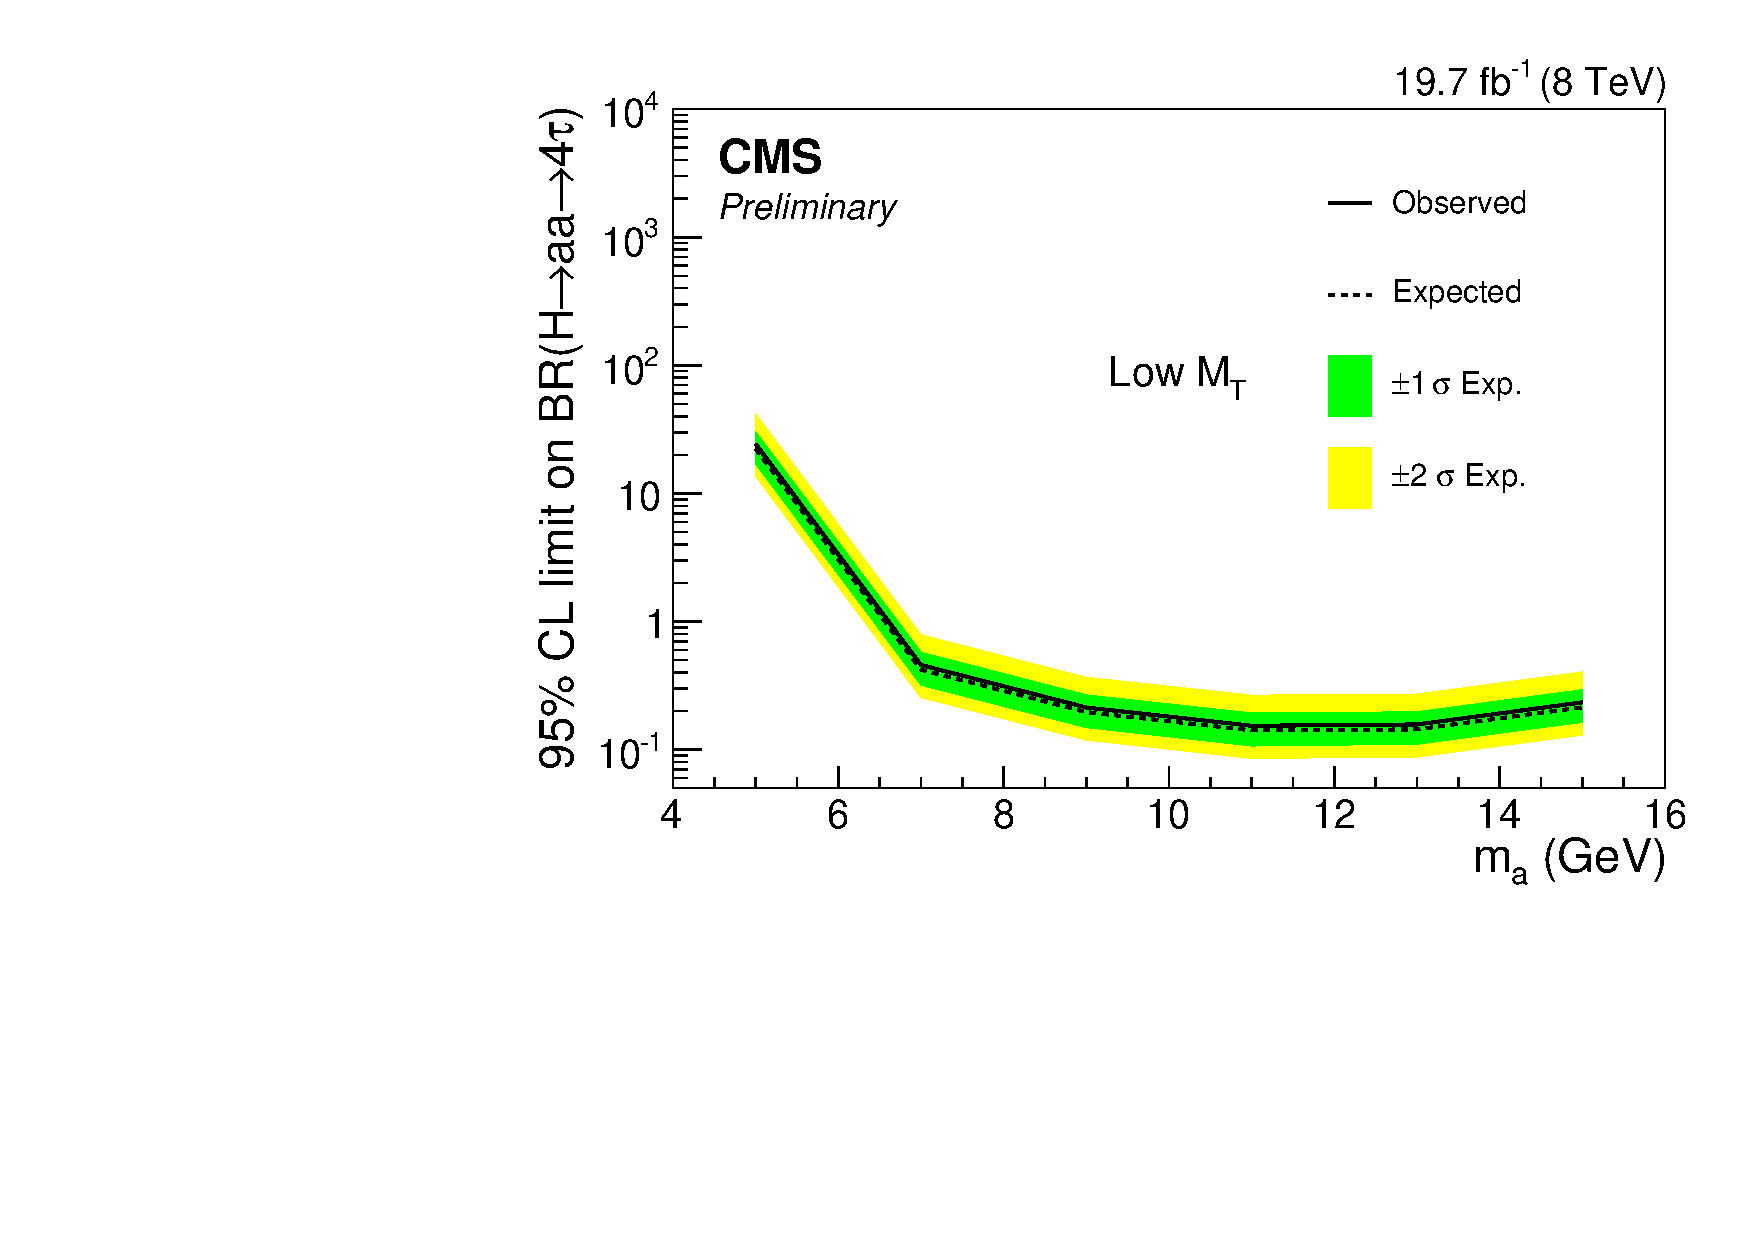
\includegraphics[width=\cmsFigWidth]{figures/expLimits_Br_lowMT_20GeV_ggHVBF}
    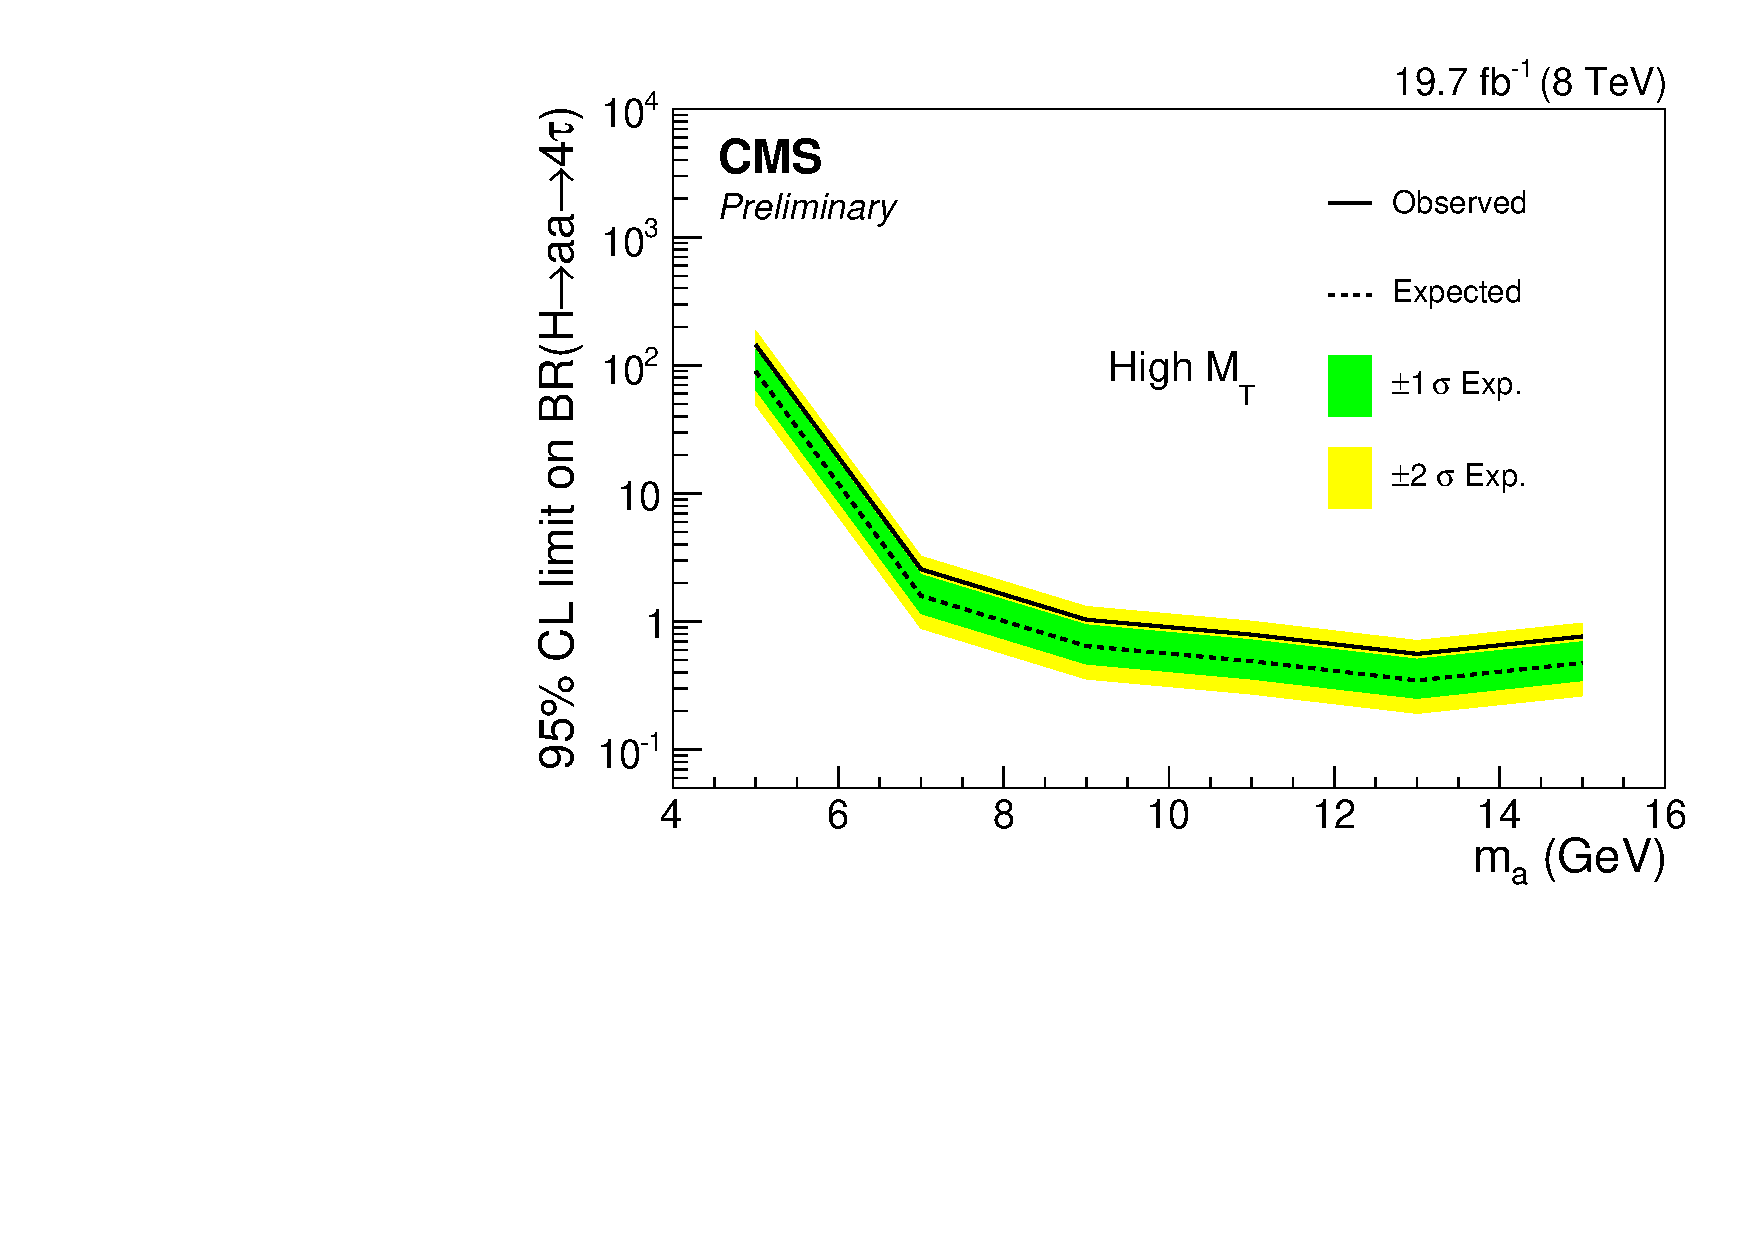
\includegraphics[width=\cmsFigWidth]{figures/expLimits_Br_highMT_20GeV_ggHWH}
    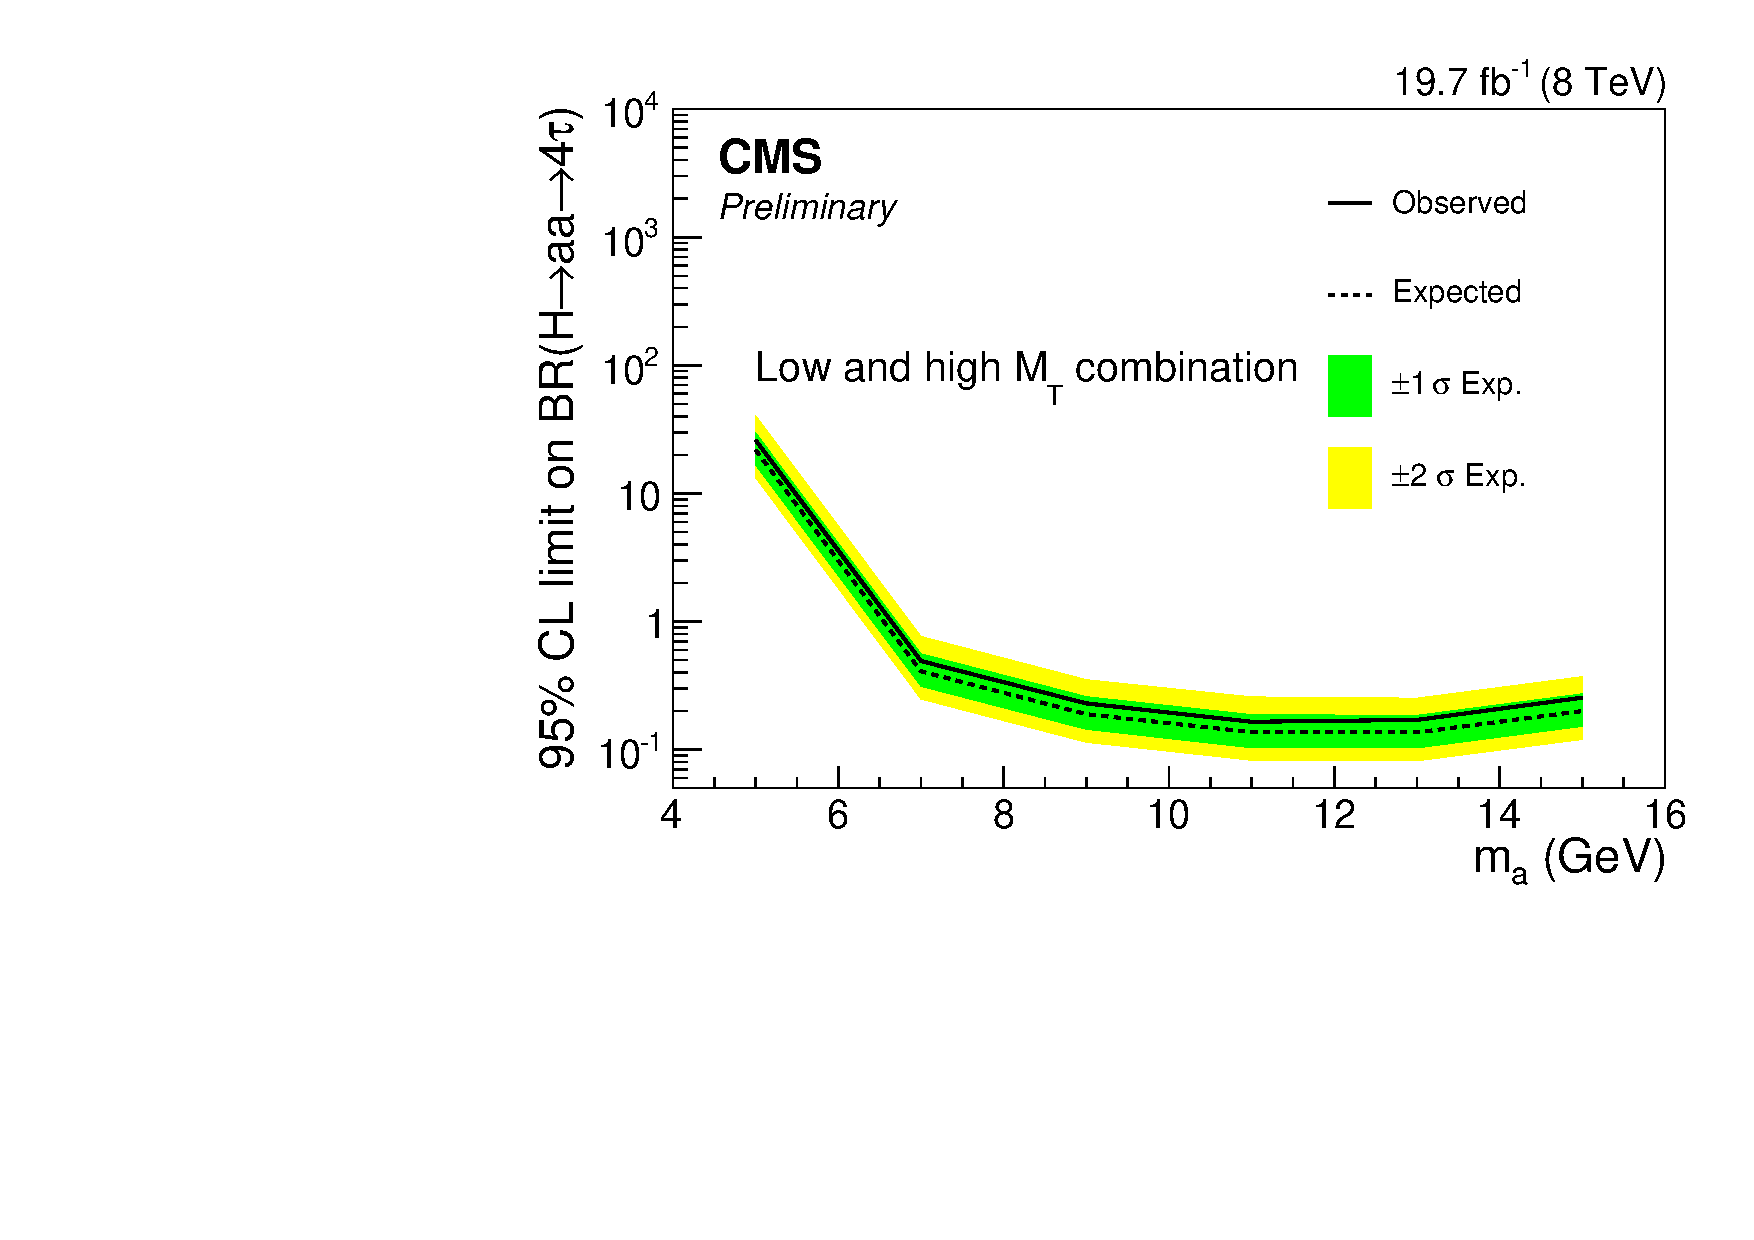
\includegraphics[width=\cmsFigWidth]{figures/expLimits_Br_20GeV_4sig}
    \caption{Observed 95\% C.L. limits (solid black curve) on the branching ratio Br($H\rightarrow$$aa\rightarrow4\tau$), compared to expected limits (dotted black curve, with $\pm1\sigma$ bands in green and $\pm2\sigma$ bands in yellow) at pseudoscalar mass points $m_{a}$ = 5 through 15 GeVcc.  (Top \cmsLeft) $M_{\text{T}}$ \textless\xspace 50 GeV. (Top \cmsRight) $M_{\text{T}}$ \textgreater\xspace 50 GeV.  (Bottom) Combined result between the low- and high-$M_{\text{T}}$ bins.}
    \label{fig:lowhighMTCLs}
  \end{center}
\end{figure}

These model-independent observed and expected $\text{CL}_{\text{s}}$ limits, expressed in terms of limits on Br($H\rightarrow$$aa\rightarrow4\tau$) assuming SM Higgs production cross-sections, are also tabulated in Tables~\ref{tab:CLs-limits-lowMT}-\ref{tab:CLs-limits}.

\begin{table*}
\begin{center}
  \caption{Observed and expected $\text{CL}_{\text{s}}$ limits on Br($H\rightarrow$$aa\rightarrow4\tau$) assuming SM Higgs production cross-sections in the low-$M_{\text{T}}$ bin.}
%\resizebox{\columnwidth}{!}{%
\singlespacing
\begin{tabular}{|m{3cm}|c|c|c|c|c|c|c|}
  \hline
  $m_{a}$ (GeV) & -2$\sigma$ & -1$\sigma$ & Median expected & +1$\sigma$ & +2$\sigma$ & Observed \\
  \hline
  \hline
  5 & 13.6 & 17.0 & 22.3 & 30.4 & 41.7 & 24.3 \\
  \hline
  7 & 0.255 & 0.318 & 0.420 & 0.576 & 0.787 & 0.457 \\
  \hline
  9 & 0.119 & 0.148 & 0.196 & 0.268 & 0.367 & 0.213 \\
  \hline
  11 & 0.0852 & 0.107 & 0.141 & 0.193 & 0.266 & 0.153 \\
  \hline
  13 & 0.0875 & 0.110 & 0.144 & 0.197 & 0.272 & 0.157 \\
  \hline
  15 & 0.130 & 0.163 & 0.214 & 0.294 & 0.404 & 0.234 \\
  \hline
  \end{tabular}%
%}
\label{tab:CLs-limits-lowMT}
\end{center}
\end{table*}

\begin{table*}
\begin{center}
  \caption{Observed and expected $\text{CL}_{\text{s}}$ limits on Br($H\rightarrow$$aa\rightarrow4\tau$) assuming SM Higgs production cross-sections in the high-$M_{\text{T}}$ bin.}
%\resizebox{\columnwidth}{!}{%
\singlespacing
\begin{tabular}{|m{3cm}|c|c|c|c|c|c|c|}
  \hline
  $m_{a}$ (GeV) & -2$\sigma$ & -1$\sigma$ & Median expected & +1$\sigma$ & +2$\sigma$ & Observed \\
  \hline
  \hline
  5 & 49.2 & 64.7 & 89.6 & 132 & 186 & 145 \\
  \hline
  7 & 0.883 & 1.15 & 1.59 & 2.33 & 3.23 & 2.56 \\
  \hline
  9 & 0.355 & 0.465 & 0.643 & 0.942 & 1.31 & 1.03 \\
  \hline
  11 & 0.271 & 0.355 & 0.490 & 0.719 & 1.005 & 0.789 \\
  \hline
  13 & 0.192 & 0.251 & 0.347 & 0.508 & 0.711 & 0.559 \\
  \hline
  15 & 0.262 & 0.345 & 0.475 & 0.696 & 0.973 & 0.765 \\
  \hline
  \end{tabular}%
%}
\label{tab:CLs-limits-highMT}
\end{center}
\end{table*}

\begin{table*}
\begin{center}
  \caption{Observed and expected $\text{CL}_{\text{s}}$ limits on Br($H\rightarrow$$aa\rightarrow4\tau$) assuming SM Higgs production cross-sections for the combination of the low- and high-$M_{\text{T}}$ bins.}
%\resizebox{\columnwidth}{!}{%
\singlespacing
\begin{tabular}{|m{3cm}|c|c|c|c|c|c|c|}
  \hline
  $m_{a}$ (GeV) & -2$\sigma$ & -1$\sigma$ & Median expected & +1$\sigma$ & +2$\sigma$ & Observed \\
  \hline
  \hline
  5 & 13.2 & 16.7 & 21.8 & 29.7 & 40.4 & 26.0 \\
  \hline
  7 & 0.248 & 0.312 & 0.408 & 0.560 & 0.765 & 0.491 \\
  \hline
  9 & 0.114 & 0.144 & 0.189 & 0.259 & 0.352 & 0.230 \\
  \hline
  11 & 0.0825 & 0.103 & 0.137 & 0.187 & 0.258 & 0.165 \\
  \hline
  13 & 0.0817 & 0.103 & 0.136 & 0.185 & 0.252 & 0.171 \\
  \hline
  15 & 0.120 & 0.152 & 0.200 & 0.273 & 0.371 & 0.254 \\
  \hline
  \end{tabular}%
%}
\label{tab:CLs-limits}
\end{center}
\end{table*}